\documentclass[tikz,border=6pt]{standalone}
\usepackage[dvipsnames]{xcolor}
\usepackage{amsmath,amssymb}
\usetikzlibrary{calc,positioning,shapes.geometric}

% Color palette
\colorlet{leftdraw}{RoyalBlue}
\colorlet{leftfill}{RoyalBlue!18}
\colorlet{rightdraw}{Magenta}
\colorlet{rightfill}{Apricot!70}
\colorlet{corefill}{MidnightBlue!85}
\colorlet{overtext}{RoyalBlue!60!black}

% Styles
\tikzset{
  venn/ellipse/.style={line width=1pt},
  leftzone/.style={draw=leftdraw, fill=leftfill, fill opacity=0.72},
  rightzone/.style={draw=rightdraw, fill=rightfill, fill opacity=0.72},
  corezone/.style={fill=corefill, draw=none, fill opacity=0.95},
  title/.style={font=\normalsize},
  labelL/.style={text=leftdraw, font=\small},
  labelR/.style={text=rightdraw, font=\small},
  faint/.style={text=overtext, font=\small}
}

\begin{document}
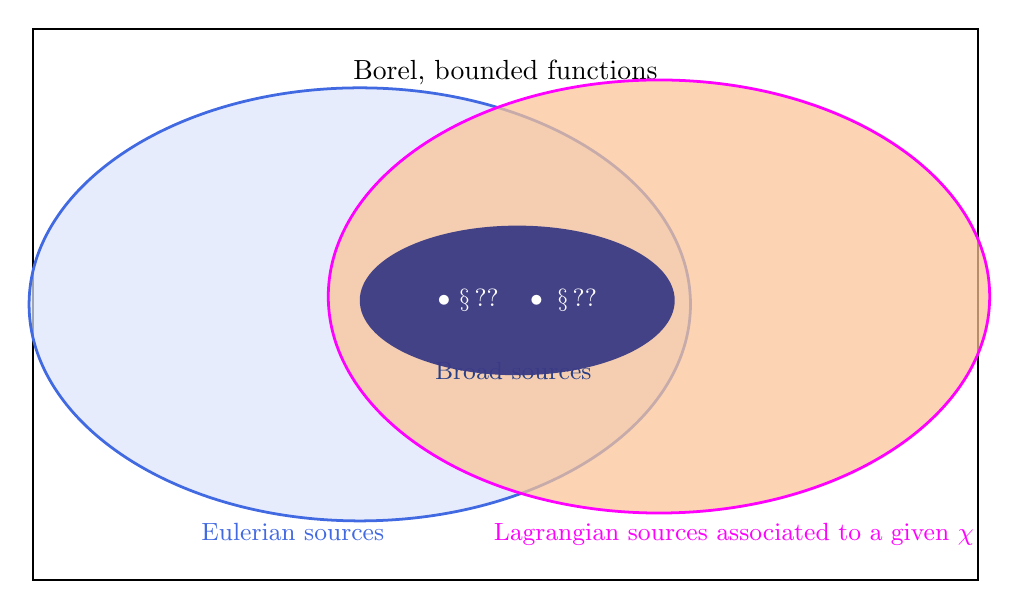
\begin{tikzpicture}[x=1cm,y=1cm]
  % Frame (12 cm x 7 cm)
  \draw[line width=.8pt] (0,0) rectangle (12,7);

  % Title
  \node[title] at (6,6.45) {Borel, bounded functions};

  % Two large overlapping ellipses
  \draw[leftzone, venn/ellipse]  (4.15,3.5) ellipse (4.2 and 2.75);
  \draw[rightzone, venn/ellipse] (7.95,3.6) ellipse (4.2 and 2.75);

  % Overlap label
  \node[faint] at (6.1,2.65) {Broad sources};

  % Dark core ellipse inside the overlap
  \fill[corezone] (6.15,3.55) ellipse (2 and .95);
  \node[text=white, font=\small] at (6.15,3.55)
    {$\bullet\ \S\,??\quad\bullet\ \S\,??$};

  % Captions
  \node[labelL, anchor=north] at (3.3,.85) {Eulerian sources};
  \node[labelR, anchor=north] at (8.9,.85)
    {Lagrangian sources associated to a given $\chi$};
\end{tikzpicture}
\end{document}